\chapter{Grundlagen}
\label{ch:Grundlagen}


UDP

Beim User Datagram Protocol handelt es sich um ein verbindungsloses und in jeglicher Hinsicht ungeschütztes Protokoll, das auf der Transportebene (Schicht 4 im OSI-Schichtenmodell) arbeitet. Es bestehen keinerlei Mechanismen, die das korrekte Übertragen von Paketen gewährleisten. Hierzu zählen:

\begin{description}
	\item[Sicherheit] Die Sicherheit, dass Pakete überhaupt ankommen
	\item[Reihenfolge] Die Reihenfolge, in der Pakete ankommen
	\item[FlowControl] Ein Überlaufschutz des Empfängerspeichers (FlowControl)
	\item[CongestionControl] Stauvermeidung in der Übertragungskette (CongestionControl)
	\item[Angriffe] Schutz gegen Paketmanipulation von dritten
\end{description}

\begin{figure}
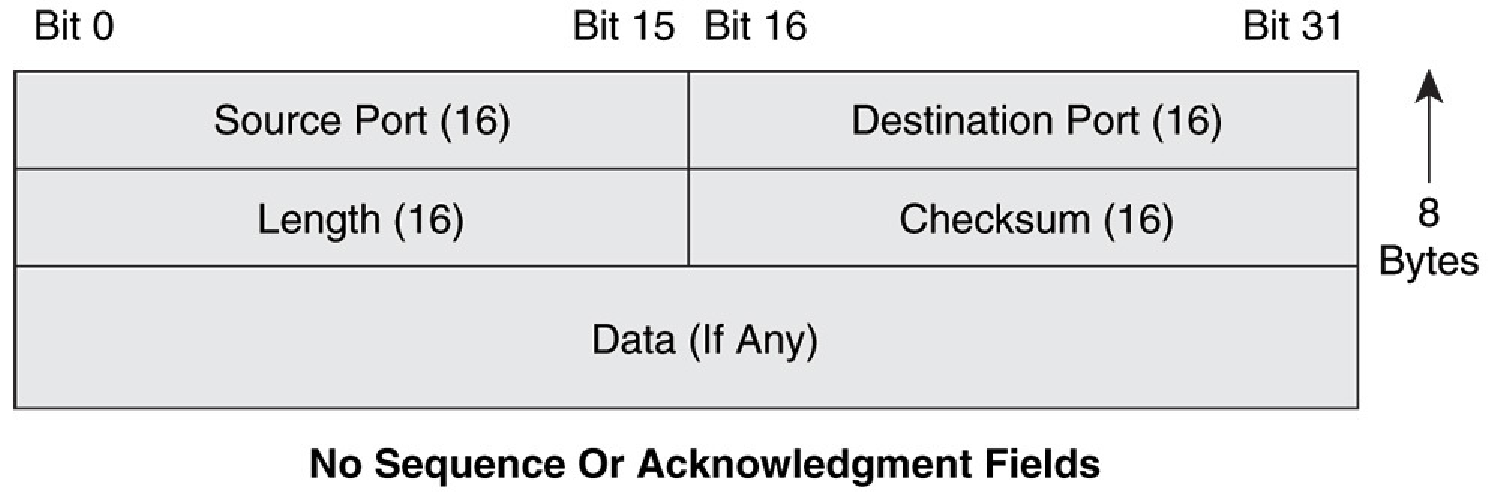
\includegraphics[width=\textwidth]{images/UDP_header.pdf}
\caption{UDP Header}
\label{fig:udp_header}
\end{figure}

Ein UDP Header besteht aus 8 Byte. Mit diesen 8 Byte werden lediglich Source-Port, Destination-Port, Länge und die Checksumme übertragen. Dieser vergleichsweise kleine Header (vgl. TCP mit etwa 20 Byte), führt zu einem geringen Overhead während der Übertragung, auch bei kleinen Paketen. Nachdem ein Paket gesendet wurde erfolgt keine Bestätigung des Pakets vom Empfänger. Durch diesen Uni-Direktionalen Sendevorgang entsteht wenig Traffic im Netzwerk. Falls gewisse Sicherheitsmechanismen gewünscht sind, müssen diese in höheren Schichten implementiert werden. \\
Aufgrund dieser Eigenschaften wird UDP in Bereichen eingesetzt, in denen es auf hohe Übertragungsgeschwindigkeit ankommt und eventuelle Paketverluste zu verkraften sind, bzw. von höheren Schichten aufgelöst werden.

